% TO-DO:
% * C-H-i 意义 - update content
% * relation with AI - stress significance
% * several slides can be deleted

\documentclass[16pt]{beamer}

\ifdefined\chinchin
\usepackage[CJKspace]{xeCJK}
%\setCJKmainfont[BoldFont=SimHei,ItalicFont=AR PL KaitiM GB]{Alibaba PuHuiTi}
\setCJKmainfont{Alibaba PuHuiTi}
\newcommand{\cc}[2]{#1}
\else
\newcommand{\cc}[2]{#2}
\fi

%\usepackage{newtxtext,newtxmath}	% use Times Roman font
%\usepackage{newtxtext}
%\renewcommand{\familydefault}{\sfdefault}
%\usefonttheme{serif}
\usefonttheme{professionalfonts}
%\setbeamertemplate{theorems}[numbered]
\setbeamertemplate{caption}{\insertcaption} 	% no `Figure' prefix before caption

\mode<presentation> {

%\usetheme{default}
%\usetheme{AnnArbor}
%\usetheme{Antibes}
%\usetheme{Bergen}
%\usetheme{Berkeley}
%\usetheme{Berlin}
%\usetheme{Boadilla}
%\usetheme{CambridgeUS}
%\usetheme{Copenhagen}
%\usetheme{Darmstadt}
%\usetheme{Dresden}
%\usetheme{Frankfurt}
%\usetheme{Goettingen}
%\usetheme{Hannover}
%\usetheme{Ilmenau}
%\usetheme{JuanLesPins}
%\usetheme{Luebeck}
\usetheme{Madrid}
%\usetheme{Malmoe}
%\usetheme{Marburg}
%\usetheme{Montpellier}
%\usetheme{PaloAlto}
%\usetheme{Pittsburgh}
%\usetheme{Rochester}
%\usetheme{Singapore}
%\usetheme{Szeged}
%\usetheme{Warsaw}

%\usecolortheme{albatross}
%\usecolortheme{beaver}
%\usecolortheme{beetle}
%\usecolortheme{crane}
%\usecolortheme{dolphin}
%\usecolortheme{dove}
%\usecolortheme{fly}
%\usecolortheme{lily}
\usecolortheme{orchid}
%\usecolortheme{rose}
%\usecolortheme{seagull}
%\usecolortheme{seahorse}
%\usecolortheme{whale}
%\usecolortheme{wolverine}		% Hofstra

%\setbeamertemplate{footline} % To remove the footer line in all slides uncomment this line
\setbeamertemplate{footline}[page number] % To replace the footer line in all slides with a simple slide count uncomment this line
\setbeamertemplate{navigation symbols}{} % To remove the navigation symbols from the bottom of all slides uncomment this line
}

\setbeamertemplate{headline}{}
\setbeamersize{text margin left=1mm,text margin right=1mm} 
\settowidth{\leftmargini}{\usebeamertemplate{itemize item}}
\addtolength{\leftmargini}{\labelsep}

\usepackage[backend=biber,style=numeric]{biblatex}
\bibliography{../AGI-book}
\renewcommand*{\bibfont}{\footnotesize}
\setbeamertemplate{bibliography item}[text]

\usepackage{graphicx} % Allows including images
\usepackage{tikz-cd}
\usepackage[export]{adjustbox}% http://ctan.org/pkg/adjustbox
\usepackage{verbatim} % comments
% \usepackage{tikz-cd}  % commutative diagrams
% \newcommand{\tikzmark}[1]{\tikz[overlay,remember picture] \node (#1) {};}
% \usepackage{booktabs} % Allows the use of \toprule, \midrule and \bottomrule in tables
% \usepackage{amssymb}  % \leftrightharpoons
% \usepackage{wasysym} % frownie face
% \usepackage{newtxtext,newtxmath}	% Times New Roman font
% \usepackage{sansmath}

\newcommand{\emp}[1]{{\color{violet}#1}}
\newcommand{\vect}[1]{\boldsymbol{#1}}
\newcommand{\tab}{\hspace*{1cm}}
\newcommand*\confoundFace{$\vcenter{\hbox{\includegraphics[scale=0.2]{../confounded-face.jpg}}}$}
\newcommand{\smiley}{$\vcenter{\hbox{\includegraphics[scale=0.05]{../smiling-face.png}}}$}

%%%%%%%% Make table of contents %%%%%%%

\makeatletter
\renewcommand{\boxed}[1]{\fbox{\m@th$\displaystyle\scalebox{0.9}{#1}$} \,}
\makeatother
\newif\ifframeinlbf
\frameinlbftrue
\makeatletter
\newcommand\listofframes{\@starttoc{lbf}}
\makeatother
\addtobeamertemplate{frametitle}{}{%
	\ifframeinlbf
	\addcontentsline{lbf}{section}{\protect\makebox[2em][l]{%
			\protect\usebeamercolor[fg]{structure}\insertframenumber\hfill}%
		\insertframetitle\par}%
	\else\fi
}

%----------------------------------------------------------------------------------------
%	TITLE PAGE
%----------------------------------------------------------------------------------------

\title[Structure of logic once more]{Supplement 2: \\ \vspace*{0.3cm} \cc{再谈一次 AI 的逻辑结构}
{\Huge《AI and the structure of logic, once more》}}
\author{\cc{YKY 甄景贤}{YKY}} % Your name
%\institute[] % Your institution as it will appear on the bottom of every slide, may be shorthand to save space
%{
%Independent researcher, Hong Kong \\ % Your institution for the title page
%\medskip
%\textit{generic.intelligence@gmail.com} % Your email address
%}
\date{\today} % Date, can be changed to a custom date

\begin{document}

\frameinlbffalse
\addtocounter{page}{-1}
\begin{frame}[plain,noframenumbering]
\titlepage
\end{frame}

\addtocounter{page}{-1}
\begin{frame}[noframenumbering]
\frametitle{Table of contents}
\listofframes
% \vspace*{0.5cm}
% 多谢 支持 \smiley
\end{frame}

%----------------------------------------------------------------------------------------
%	PRESENTATION SLIDES
%----------------------------------------------------------------------------------------

%------------------------------------------------

\frameinlbftrue

%\begin{frame}
%\frametitle{Fourier 神经网络}
%\begin{itemize}
%	\item 之前说过,需要 symmetric 神经网络。 可以用 \emp{多项式} 激活函数,得出一大堆 多项式的 weight-sharing 条件。 这方法在 层数 增大时,计算变得很复杂。 这是一个 computational invariant theory 的问题,我暂时未有时间深入研究
%	
%	\item 另一个方法我称之为 Fourier 神经网络
%	\item 命题空间 $\mathbb{P}\mathrm{rop}$
%\end{itemize}
%\end{frame}

\begin{frame}
\frametitle{背景: 利用 invariance 加速学习}
\begin{itemize}
	\item 以前曾经说过,机器视觉 的成功,有赖於 将 视觉的几何结构 impose 在深度神经网络上
	\item 这 深度神经网络 原本是 ``free'' 的,但加了限制之后,权重空间 变小了(例如维数降低),所以学习加速了
	\item 所谓 symmetry 的意义,简单例子:「如果知道左边等於右边,那就只需计算一次」
	\item 换句话说,数学家喜欢对称性,是因为它经常可以简化计算
	\item 同理,我们想将 逻辑结构 的对称性 impose 到神经网络
	\item 实际上,可能只需要逻辑上的交换律,就可以达到 强人工智能,正如 机器视觉的成功,在於引入了 CNN 的 convolution 结构,后者只是 视觉不变性 的其中一个最显著的 invariant
	\item 现代逻辑理论非常漂亮,我花了十多年时间才弄懂,我希望将这套 逻辑-学习 理论简单讲解一下,也算功德完满了
\end{itemize}
\end{frame}

\begin{frame}
\frametitle{逻辑的 几何 与 拓扑 结构}
\begin{itemize}
\item 在经典时代,逻辑的 代数形式 可以用 Boolean algebra 表述,然而这方法只适用於 命题逻辑
\item Boolean algebra 是中学生熟悉的,类似 Venn diagram 的结构
\item 这种结构和 拓樸学 的 open sets 结构一样,所以 命题逻辑 也可以看成是一种 topology
\item 然而 predicate logic 的结构更复杂,直到最近才有比较完善的表述
\item 现代逻辑结构和 type theory 有深刻的关系,此即 Curry-Howard isomorphism
\item 现代逻辑也涉及 topos theory,那是一种由 algebraic geometry 引入的结构
\end{itemize}
\end{frame}

\begin{frame}
\frametitle{Curry-Howard isomorphism}
\begin{itemize}
	\item Curry-Howard isomorphism 是现代逻辑的 核心思想,但我初时没有留意,以致很多东西 看不懂,明白之后 豁然开朗
	
	\item 它讲的是 \emp{逻辑证明} 与 \emp{计算} 之间的深刻关系:
	\begin{eqnarray}
	\mbox{逻辑} & \Leftrightarrow & \mbox{type theory} \\
	\mbox{逻辑证明} & \Leftrightarrow & \mbox{programs} \nonumber
	\end{eqnarray}
	% \item 程式 是一些 \emp{函数},而 神经网络 也是非线性的函数\emp{映射},所以 神经网络 也\emp{对应于} 逻辑推理
	
	\item 先看 $\Rightarrow$: 逻辑是一些 符号/形式上 的推导,所以 逻辑证明 (derivations) 必然对应於某种 计算 (computation),这很容易理解
	
	\item 再看 $\Leftarrow$: 当人们企图定义 普遍的计算模式 (models of computation) 时,发觉 总是对应於 某些逻辑; 这一点比较神秘,我也不完全了解
\end{itemize}
\end{frame}

\begin{frame}
\frametitle{Type theory}
\begin{itemize}
	\item 首先了解一下 type theory, 它起源於 Bertrand Russell 为了避开 数理逻辑上的 悖论 (paradox) 的尝试

	\item 后来发现 type thoery 用来定义 \emp{programs} 很有用

	\item 大家都知道 Lisp 语言没有 types,它是一种 untyped $\lambda$-calculus

	\item 在 Lisp 之上引入 type system,衍生成 ML, Caml, OCaml, Haskell, 等 一系列的语言

	\item 每一个 program 属於某个 type,例如 $\mathrm{length}()$ 函数:
	\begin{equation}
	\mathrm{length} : \mathsf{String} \rightarrow \mathsf{Integer}
	\end{equation}
	它输入一个 字串,输出一个 整数(字串的长度)
\end{itemize}
\end{frame}

\begin{frame}
\frametitle{Curry-Howard isomorphism 的一些细节}
\begin{itemize}
	\item 例如 我们定义一个函数 $f$, 由 $A$ 类 映射到 $B$ 类:
	\begin{equation}
	f: A \rightarrow B
	\end{equation}

	\item 这对应於 逻辑上「A 蕴涵 B」的关系:
	\begin{equation}
	A \Rightarrow B
	\end{equation}
	
	\item \cc{逻辑上,每个命题 $A$ 都有一个 \emp{proof object} 或 \emp{witness}, 记作 $\square : A$}
	{In logic, for each proposition $A$ would be associated a \emp{proof object} or \emp{witness} $\square : A$}

	\item 而函数 $f$ 就是将 $a:A$ (A 的证明)映射到 $b:B$ (B 的证明):
	\begin{equation}
	f: a \mapsto b
	\end{equation}

	\item 类似地,有函数可以将 两个分开的命题 $A$ 和 $B$ 的证明 映射到 $A \wedge B$ 的证明,这里不赘述了
	
	\item 简言之,可以建立 \emp{命题逻辑} 的 $\Rightarrow, \wedge, \vee, \neg$ 对应到一些函数上,这些函数用 typed $\lambda$-calculus 定义
	
	\item 但与 $\lambda$-calculus 对应的逻辑 没有 \emp{排中律},它是 intuitionistic logic.  这种逻辑 符合 数学上的 构造主义 (constructivism)
\end{itemize}
\end{frame}

\begin{frame}
\frametitle{谓词逻辑 (predicate logic)}
\begin{itemize}
	\item 刚才说明了,type theory 对应於 \emp{命题逻辑}
	
	\item 如果要处理 predicates,需要一些 特殊的 types
	
	\item Predicate 就是有「洞」的命题,填入某些 objects 之后变成真正的命题
	
	\item 换句话说 predicate $P$ 是一个函数 $P: X \rightarrow \mathcal{U}$,对每个 $x$ 产生 $P(x)$,这 $P(x)$ 也是一个 type, 而 $\mathcal{U}$ 是所有 types 的 universe

	\item 这样会产生一些不是很像「命题」的 types,例如 自然数的类 $\mathbb{N}$, 似乎不是命题; 关於这点我暂时仍不太清楚

	\item 重点是: type theory 很自然地 \emp{同构}於 categories,with objects = types and morphisms = function types ($A \rightarrow B$)
	
	\item 而在 categories 中,predicate 的结构可以用 \emp{fibration} 描述,记作
	$\mathrel{\substack{\mathbf{Pred}\\\downarrow\\\mathbf{Set}}}$
	
	\item Fibrations 符合某种 universal property,是由 代数几何/拓扑 借来的概念
\end{itemize}
\end{frame}

\begin{frame}
\frametitle{Curry-Howard isomorphism 的意义}
\begin{itemize}
	\item 有些逻辑学家 察觉到 类型论 的 $A \rightarrow B$ 和逻辑中 $A \Rightarrow B$ 是一模一样的

	\item 这个关系的 发现者 至少包括:  Brouwer-Heyting-Kolmogorov-Sch\"{o}nfinkel-Curry-Meredith-Kleene-Feys-G\"{o}del-L\"{a}uchli-Kreisel-Tait-Lawvere-Howard-\mbox{de Bruijn}-Scott-Martin-L\"{o}f-Girard-Reynolds-Stenlund-Constable-Coquand-Huet-....

	\item C-H 同构 的深刻之处,在於把 符号逻辑上的 proofs 和 程序语言 的 programs 划上等号,前者是 符号/静态的,后者是 程序/动态的

	\item 每个 proof 就是一个 program,它输入一些 arguments,输出 关於那些 arguments 的证明
	
	\item 例如: 「所有人都会死」是一个 program,它输入「苏格拉底」,输出「苏格拉底会死」 
	
	\item 我发现 这个对应 也可以应用到 深度学习: 神经网络 也是一種 函數 / mapping,它将 逻辑前提 map 到结论
\end{itemize}
\end{frame}

\begin{frame}
\frametitle{Topos theory and fibrations}
\begin{itemize}
	\item Predicate logic (谓词逻辑)和 命题逻辑 之间的差异在於 fibration 结构
	\item Fibration 通常用 $\mathrel{\substack{\mathbb{E}\\\downarrow \\\mathbb{B}}  {\scriptstyle \pi}}$ 表示,$\mathbb{B}$ = base space, $\mathbb{E}$ = \`{e}tal\`{e} space, $\pi$ = projection
	\item 例如 base space 是一个 base set, \`{e}tale space 是这个集合上的 predicates
	\item 由於 Curry-Howard 对应, type = propositions,在 base 空间上只有 命题逻辑
	\item 例如 $\mathbb{B}$ 空间的一个 type 是 $\mathrm{Human}$,$\mathbb{E}$ 空间的一个谓词是 $\mathrm{Mortal}$
	\item 於是有以下这个 type inference rule:
	\begin{equation}
	i:\mathsf{Human} \vdash \mathrm{Mortal}(i): \mathsf{Prop}
	\end{equation}
	意思是说,如果 $i$ 属於 $\mathsf{Human}$ 类型,则 $\mathrm{Mortal}(i)$ 属於 $\mathsf{Prop}$ 类型
\end{itemize}
\end{frame}


\begin{frame}[fragile]
\frametitle{Logic's topology and geometry}
\begin{itemize}
	\item 总结一下,大家 中/小学 时期 都熟悉 Venn diagrams,其实 命题逻辑 具有 \emp{拓扑}的 open sets 结构:
	\begin{equation}
	\vcenter{\hbox{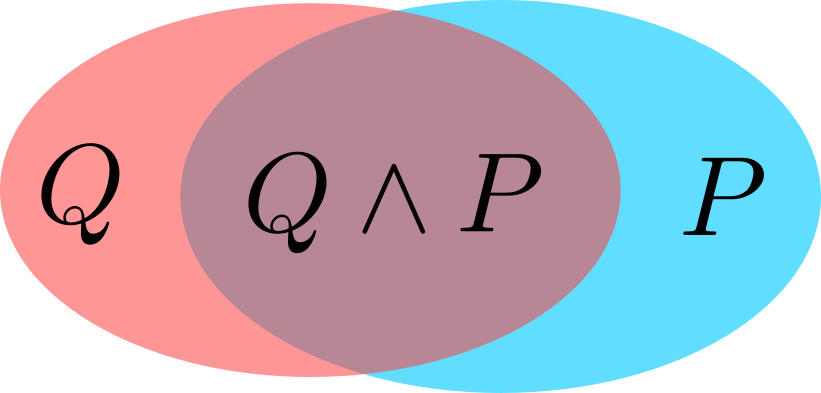
\includegraphics[scale=0.4]{Venn-diagram.png}}}
	\end{equation}
	而 谓词 (predicates) 是在 base set 上面的 纤维化 (fibration), 记作 $\mathrel{\substack{\mathbb{E}\\\downarrow \\\mathbb{B}}  {\scriptstyle \pi}}$
	

	\item 於是有以下的关系: ($\pi$ = fibration)
	\begin{equation}
	\begin{tikzcd}[column sep = large, row sep = large]
	\mbox{homotopy} \arrow[d, "\pi"]
	& \stackrel{\mbox{predicate}}{\mbox{logic}} \arrow[d, "\pi"]
	& \mbox{HoTT} \arrow[d, "\pi"]
	& \stackrel{\mbox{predicate}}{\mbox{logic}} \arrow[d, "\pi"]
	\\
	\mbox{topology} \arrow[r, leftrightarrow, "\cong"]
	& \stackrel{\mbox{propositional}}{\mbox{logic}} \arrow[leftrightarrow]{r}{Curry}[swap]{Howard}
	& \stackrel{\mbox{type}}{\mbox{theory}} \arrow[r, leftrightarrow, "\cong"]
	& \stackrel{\mbox{categorical}}{\mbox{logic}}
	\end{tikzcd}
	\end{equation}
	\item HoTT = homotopy type theory, 是 Voevodsky 等人提出的 非常新的理论
\end{itemize}
\end{frame}


\begin{frame}
\frametitle{HoTT (homotopy type theory)}
\begin{itemize}
	\item 2017年,提出 HoTT  的 Voevodsky 在 51岁 英年早逝
	\begin{equation}
	\vcenter{\hbox{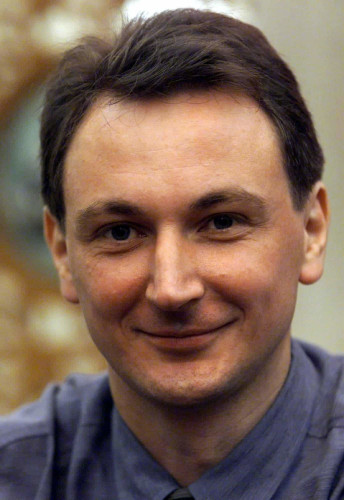
\includegraphics[scale=0.4]{Voevodsky.jpg}}}
	\end{equation}
\end{itemize}
\end{frame}

\begin{frame}[plain]
HoTT 理论我不太了解,也未知它对 AGI 有没有用,暂时留下这个 remark:
\begin{itemize}
	\item HoTT 的作用似乎是对 types 的空间作抽象的描述,例如将 types 空间分成 levels:
	\begin{itemize}
		\item \textbf{Level 0:} up to homotopy equivalence there is just one contractible space that we call ``point'' and denote $pt$
		
		\item \textbf{Level 1:} up to homotopy equivalence there are 2 spaces at this level:  the \textbf{empty space} $\varnothing$ and the \textbf{point} $pt$.  We call them \textbf{truth values}.  We also refer to types of this level as \textbf{properties} and \textbf{propositions}.  Propositional logic lives at $h$-level 1
		
		\item \textbf{Level 2:}  Types of this level are characterized by the property that their path spaces are empty or contractible.  So such types are disjoint unions of contractible components (points), or in other words \textbf{sets} of points.  This will be our working notion of sets available in this framework.
		
		\item \textbf{Level 3:}  Types of this level are characterized by the property that their path spaces are sets (up to homotopy equivalence).  These are obviously (ordinary flat) \textbf{groupoids} (with path spaces hom-sets)
		
		\item \textbf{Level 4 $... n+2$:}  Here we get 2-groupoids to $n$-groupoids
	\end{itemize}
\end{itemize}
\end{frame}

\begin{frame}[fragile]
\frametitle{逻辑 与 AI 之间的关系}
\begin{itemize}
	\item 那既然 AI 基於 逻辑,而逻辑的结构 如上所述,则 AI 与逻辑之间 必然存在 精确 (precise) 的联系

	\item BERT 似乎是在执行 句子之间的变换,而这些句子是 word embedding 的 concatenation,例如:
	\begin{equation}
	\begin{tikzcd}[column sep = large]
	\mbox{苏格拉底} \cdot \mbox{是} \cdot \mbox{人}
	\arrow[r, "BERT"]
	& \mbox{苏格拉底} \cdot \mbox{会} \cdot \mbox{死}
	\end{tikzcd}
	\end{equation}
	这个做法看似很「粗暴」,其实它和逻辑式子的作用一样:
	\begin{equation}
	\forall x. \; \mbox{Human}(x) \rightarrow \mbox{Mortal}(x)
	\end{equation}
	而这式子,根据 Curry-Howard 对应,就是上面的函数映射!

	\item 这些映射的对象,是形如 ``$a \in A$'' 这样的物体,它们有 predicates 的几何/拓扑结构,但我们现时未做到这一步,暂时只引入了 commutativity
	
	\begin{comment}
		\item 集合元素 $a$ 是 $\exists x. P(x)$ 的证明,例如 Socrates 是 $\exists x. \mbox{mortal}(x)$ 的证明
		\item 当 神经网络 \emp{调教} 某些元素的 映射 (mapping) 时,它同时在学习某个逻辑的 formula;  换句话说,逻辑 是几何空间中的映射
		\item 逻辑的 谓词 (predicates) 是在 基底元素空间上的一个 \emp{纤维丛结构} (fibration) :
		\begin{equation}
		\vcenter{\hbox{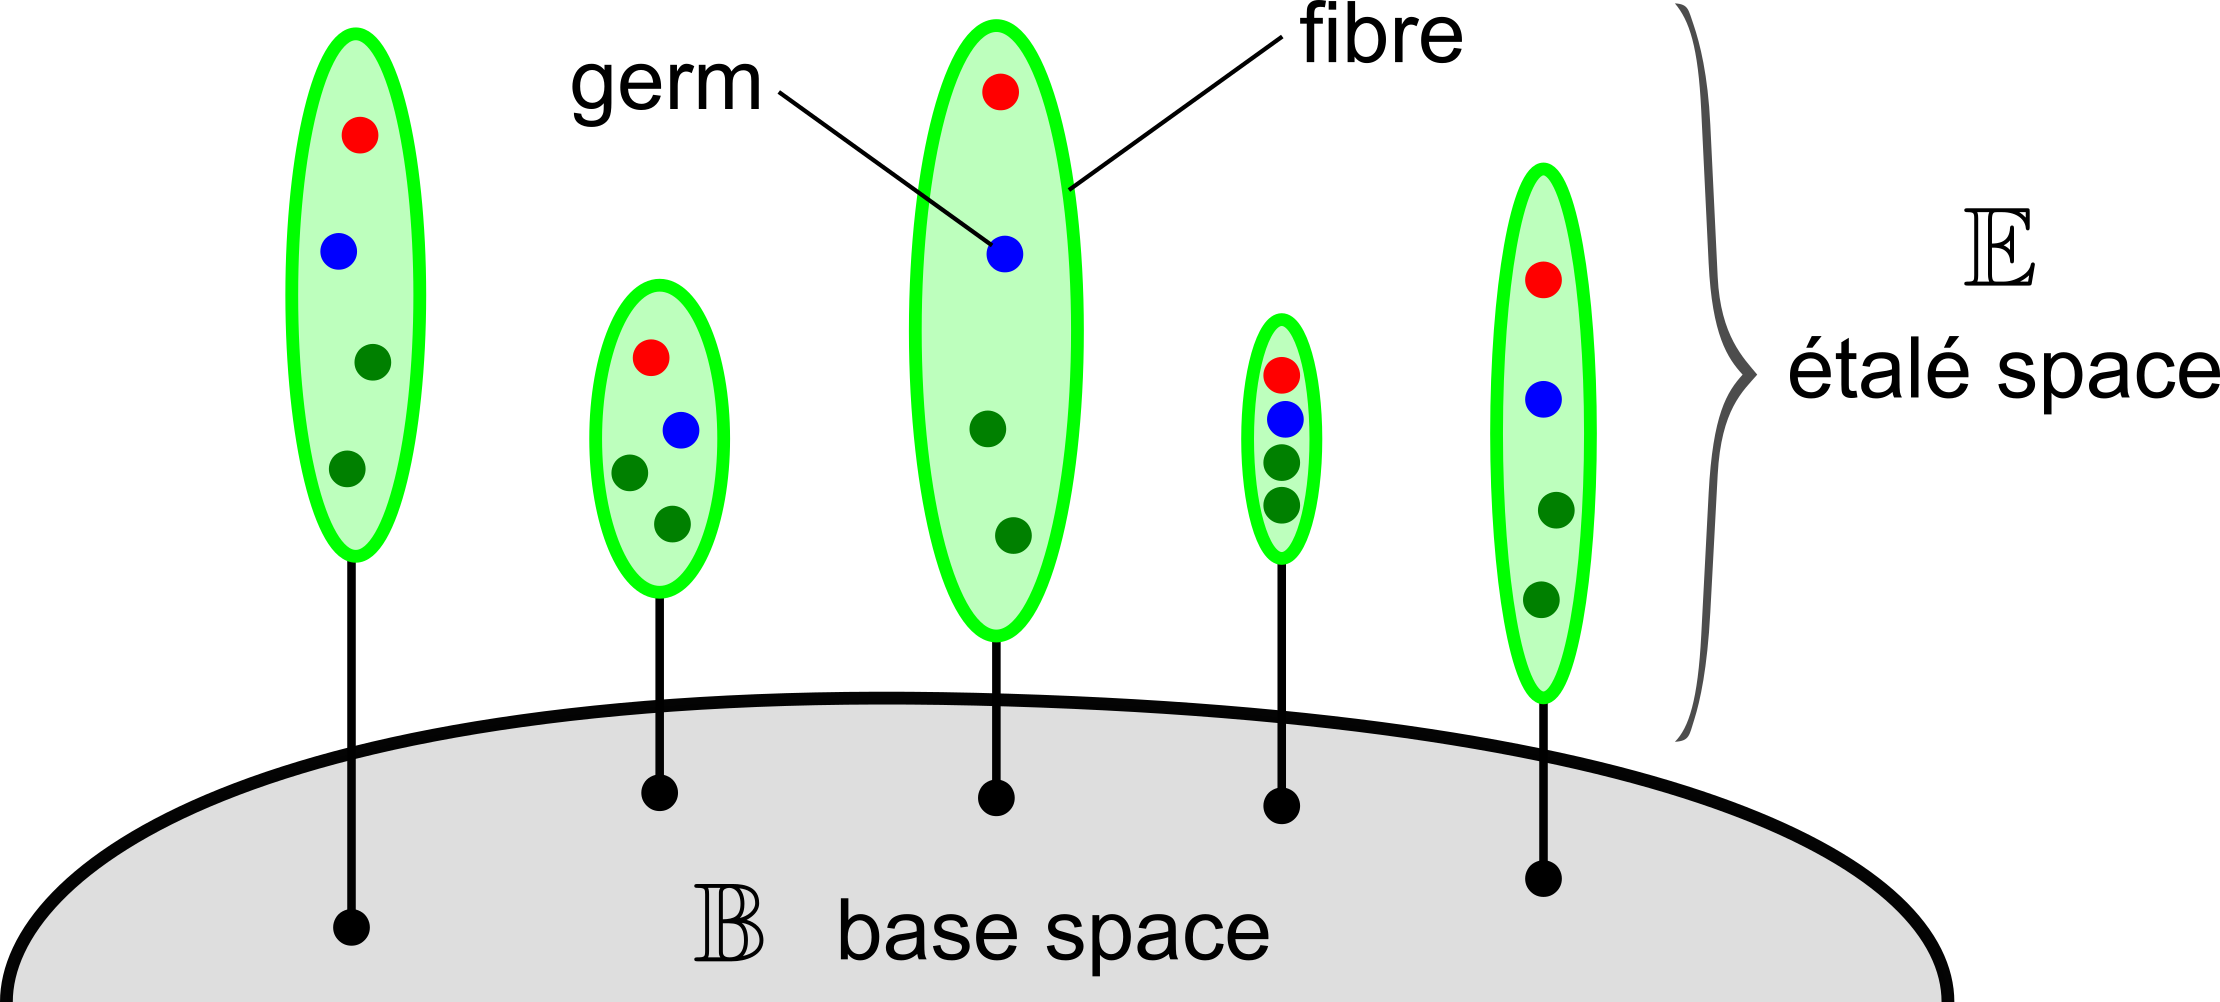
\includegraphics[scale=0.5]{etale-space.png}}}
		\end{equation}
	\end{comment}

	% \item 从 几何/拓扑 ``借'' 来的概念,演变成 topos 理论、HoTT 等

	% \item 这些漂亮的理论 不是无用的; 有需要时,可以從 邏輯 那邊借來更多的結構
	
	\item 可以说,逻辑的 几何结构 是「永恒」的,它可以指示 AGI 的 长远发展
	
	% \item $H(a)$ is a type.
	% \item $H$ is a prodicate type.
	% \item The proof of $H(a)$ may be the tuple $(a, H)$ or $a \in H$
\end{itemize}
\end{frame}

\begin{frame}
\frametitle{对 逻辑主义 的质疑}
\begin{itemize}
	\item 很多人怀疑: 人脑真的用 逻辑 思考吗?
	
	\item 其实我们每句表达的 \emp{语言},都是逻辑形式的 (logical form)
	
	\item 直觉认为,人脑 构造一些 \emp{models},再从 model 中「读出」一些结论
	
	\item 例如给定一个描述:「已婚妇人出轨,用刀刺死丈夫」
	\begin{equation}
	\vcenter{\hbox{
\includegraphics[scale=1.0]{murder-scene.png}}}
	\end{equation}
	
	\item 那么 妻子穿著什么衣服? 衣服什么颜色? 这些都是 \emp{臆想} 出来的细节,是不正确的
	
	\item 这个 model 可以有哪些细节? 答案是: 任何细节都不可以有,除非是 逻辑上蕴含的,或被逻辑 约束
	
	% \item 所以,其实所谓 ``model-based reasoning'' 并没有那么神奇,也并不一定正确,它的细节必需被 \emp{逻辑} 约束
	
	\item Model 本身可以是一些 抽象的逻辑命题 构成的,这也合理; 反而,一个有很多感官细节的 model 并不合理
	
	\item 其实人脑可能比我们想像中更接近逻辑化的结构
\end{itemize}
\end{frame}


\begin{frame}
\frametitle{「神经」知识表示}
为什么要研究 神经知识表示?
\begin{itemize}
	\item 从经典 logic-based AI 的传统,一直在使用「符号」的知识表示法

	\item 符号逻辑 很容易转换成 抽象代数/范畴论 形式(它们是同一个大家庭的「近亲」)
	
	\item 然而 或许存在 截然不同 的知识表示法? 但我们很难想像它 \emp{长什么样子}

	\item 人脑的「神经」知识表示,可以作为参考,然后再研究它和逻辑表示之间的 correspondence
\end{itemize}

\vspace*{0.4cm} 神经知识表示 的特点:
\begin{itemize}
	\item distributive(分布性)

	\item model-based (vs rule-based)

	\item \textit{in situ}(固定性)--- 例如辨认「猫」的时候,大脑中 相应的神经元被 激活,但这些 神经元 \emp{不能移动},所以「猫」的表示 也不可移动
\end{itemize}
问题是: 如果要辨认「白猫追黑猫」,「猫」的表示是固定的,则这两个「猫」表示 如何\emp{共存}於神经网络中?\\
答案很可能是: 两个「猫」\emp{交替}地 出现在 \emp{时间}上
\end{frame}

\begin{frame}
\frametitle{神经 特征簇 (feature clusters)}
例如,以「匙羹在杯中」作例子:
\begin{equation}
	\vcenter{\hbox{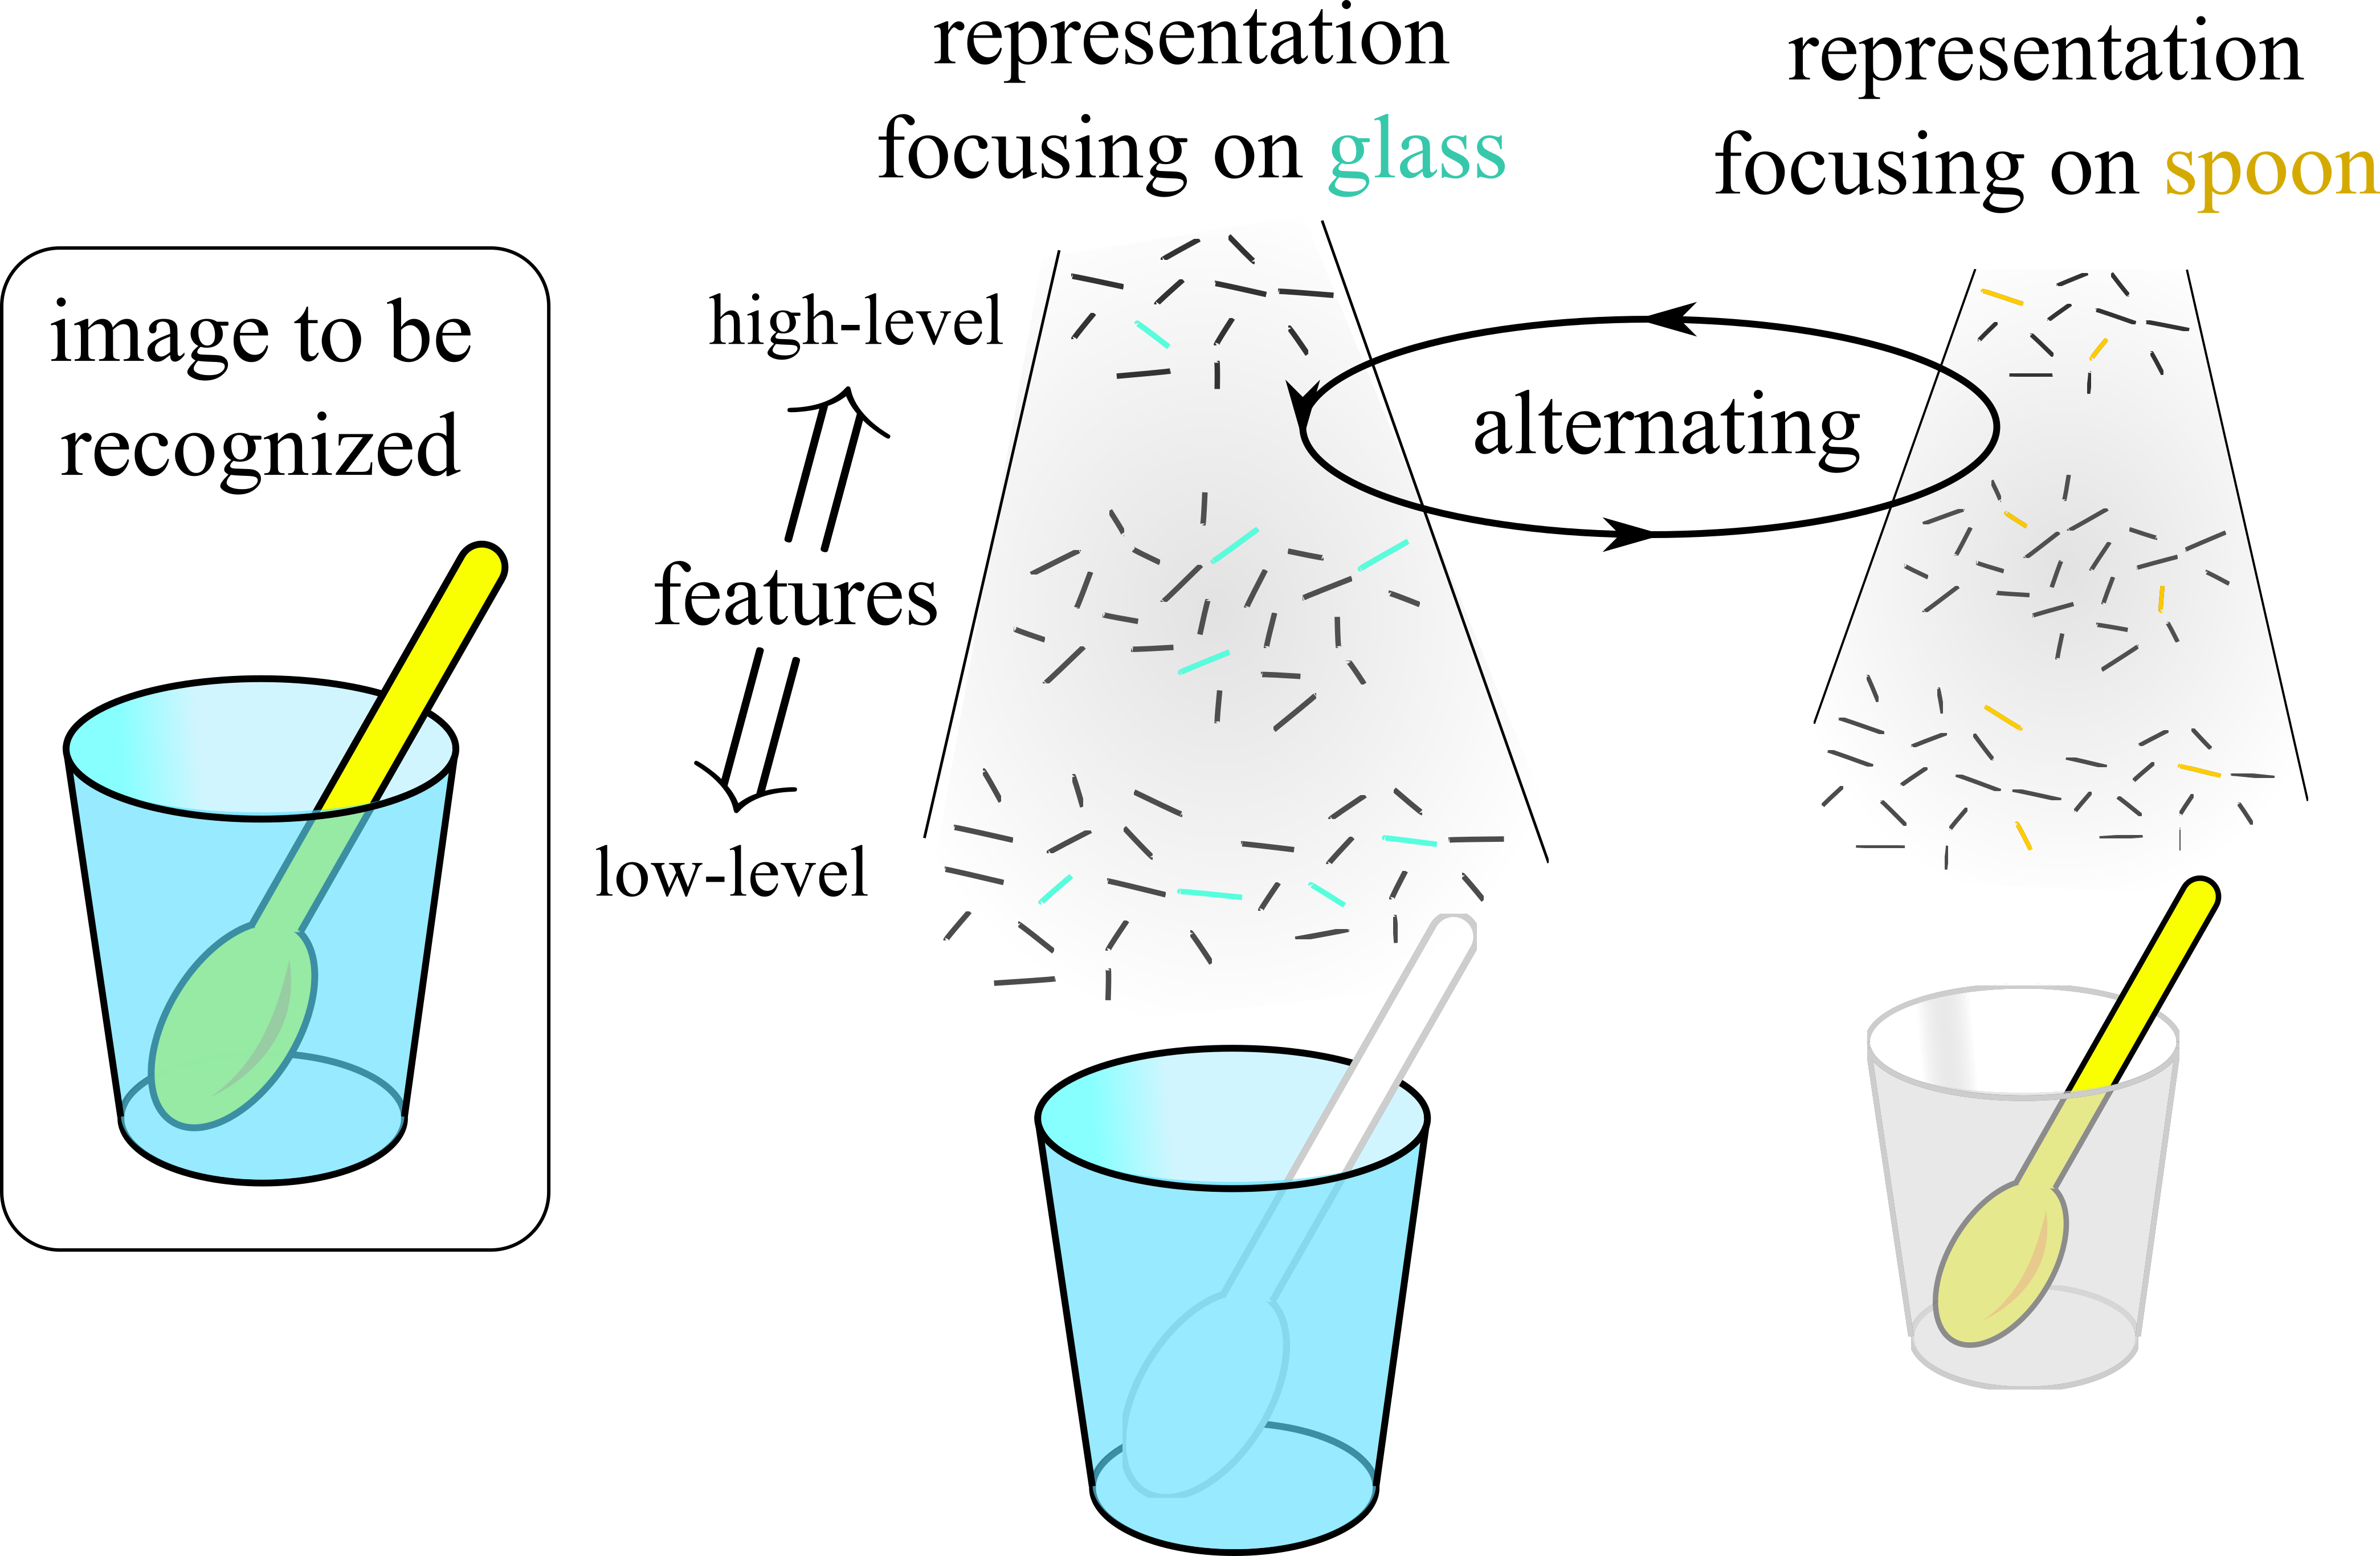
\includegraphics[scale=0.5]{neural-representation-alternating-glass-spoon.png}}}
\end{equation}
每个 复杂物体 由一个 \emp{feature cluster} 辨认。 多个「特征簇」在时间上交替出现,可以看成是一种 composition,例如 $A \cdot B$ 或 $A \circ B$.
\end{frame}

\begin{frame}
\frametitle{高阶 特徵}
\begin{itemize}
	\item 一串 特征簇 的时间序列,例如 $A \cdot B$,可以被 更\emp{高阶} 的神经网络 用作输入。 高阶辨认 的结果是一些关系 (relations),例如「匙羹\emp{在}杯\emp{内}」
	\begin{equation}
		\vcenter{\hbox{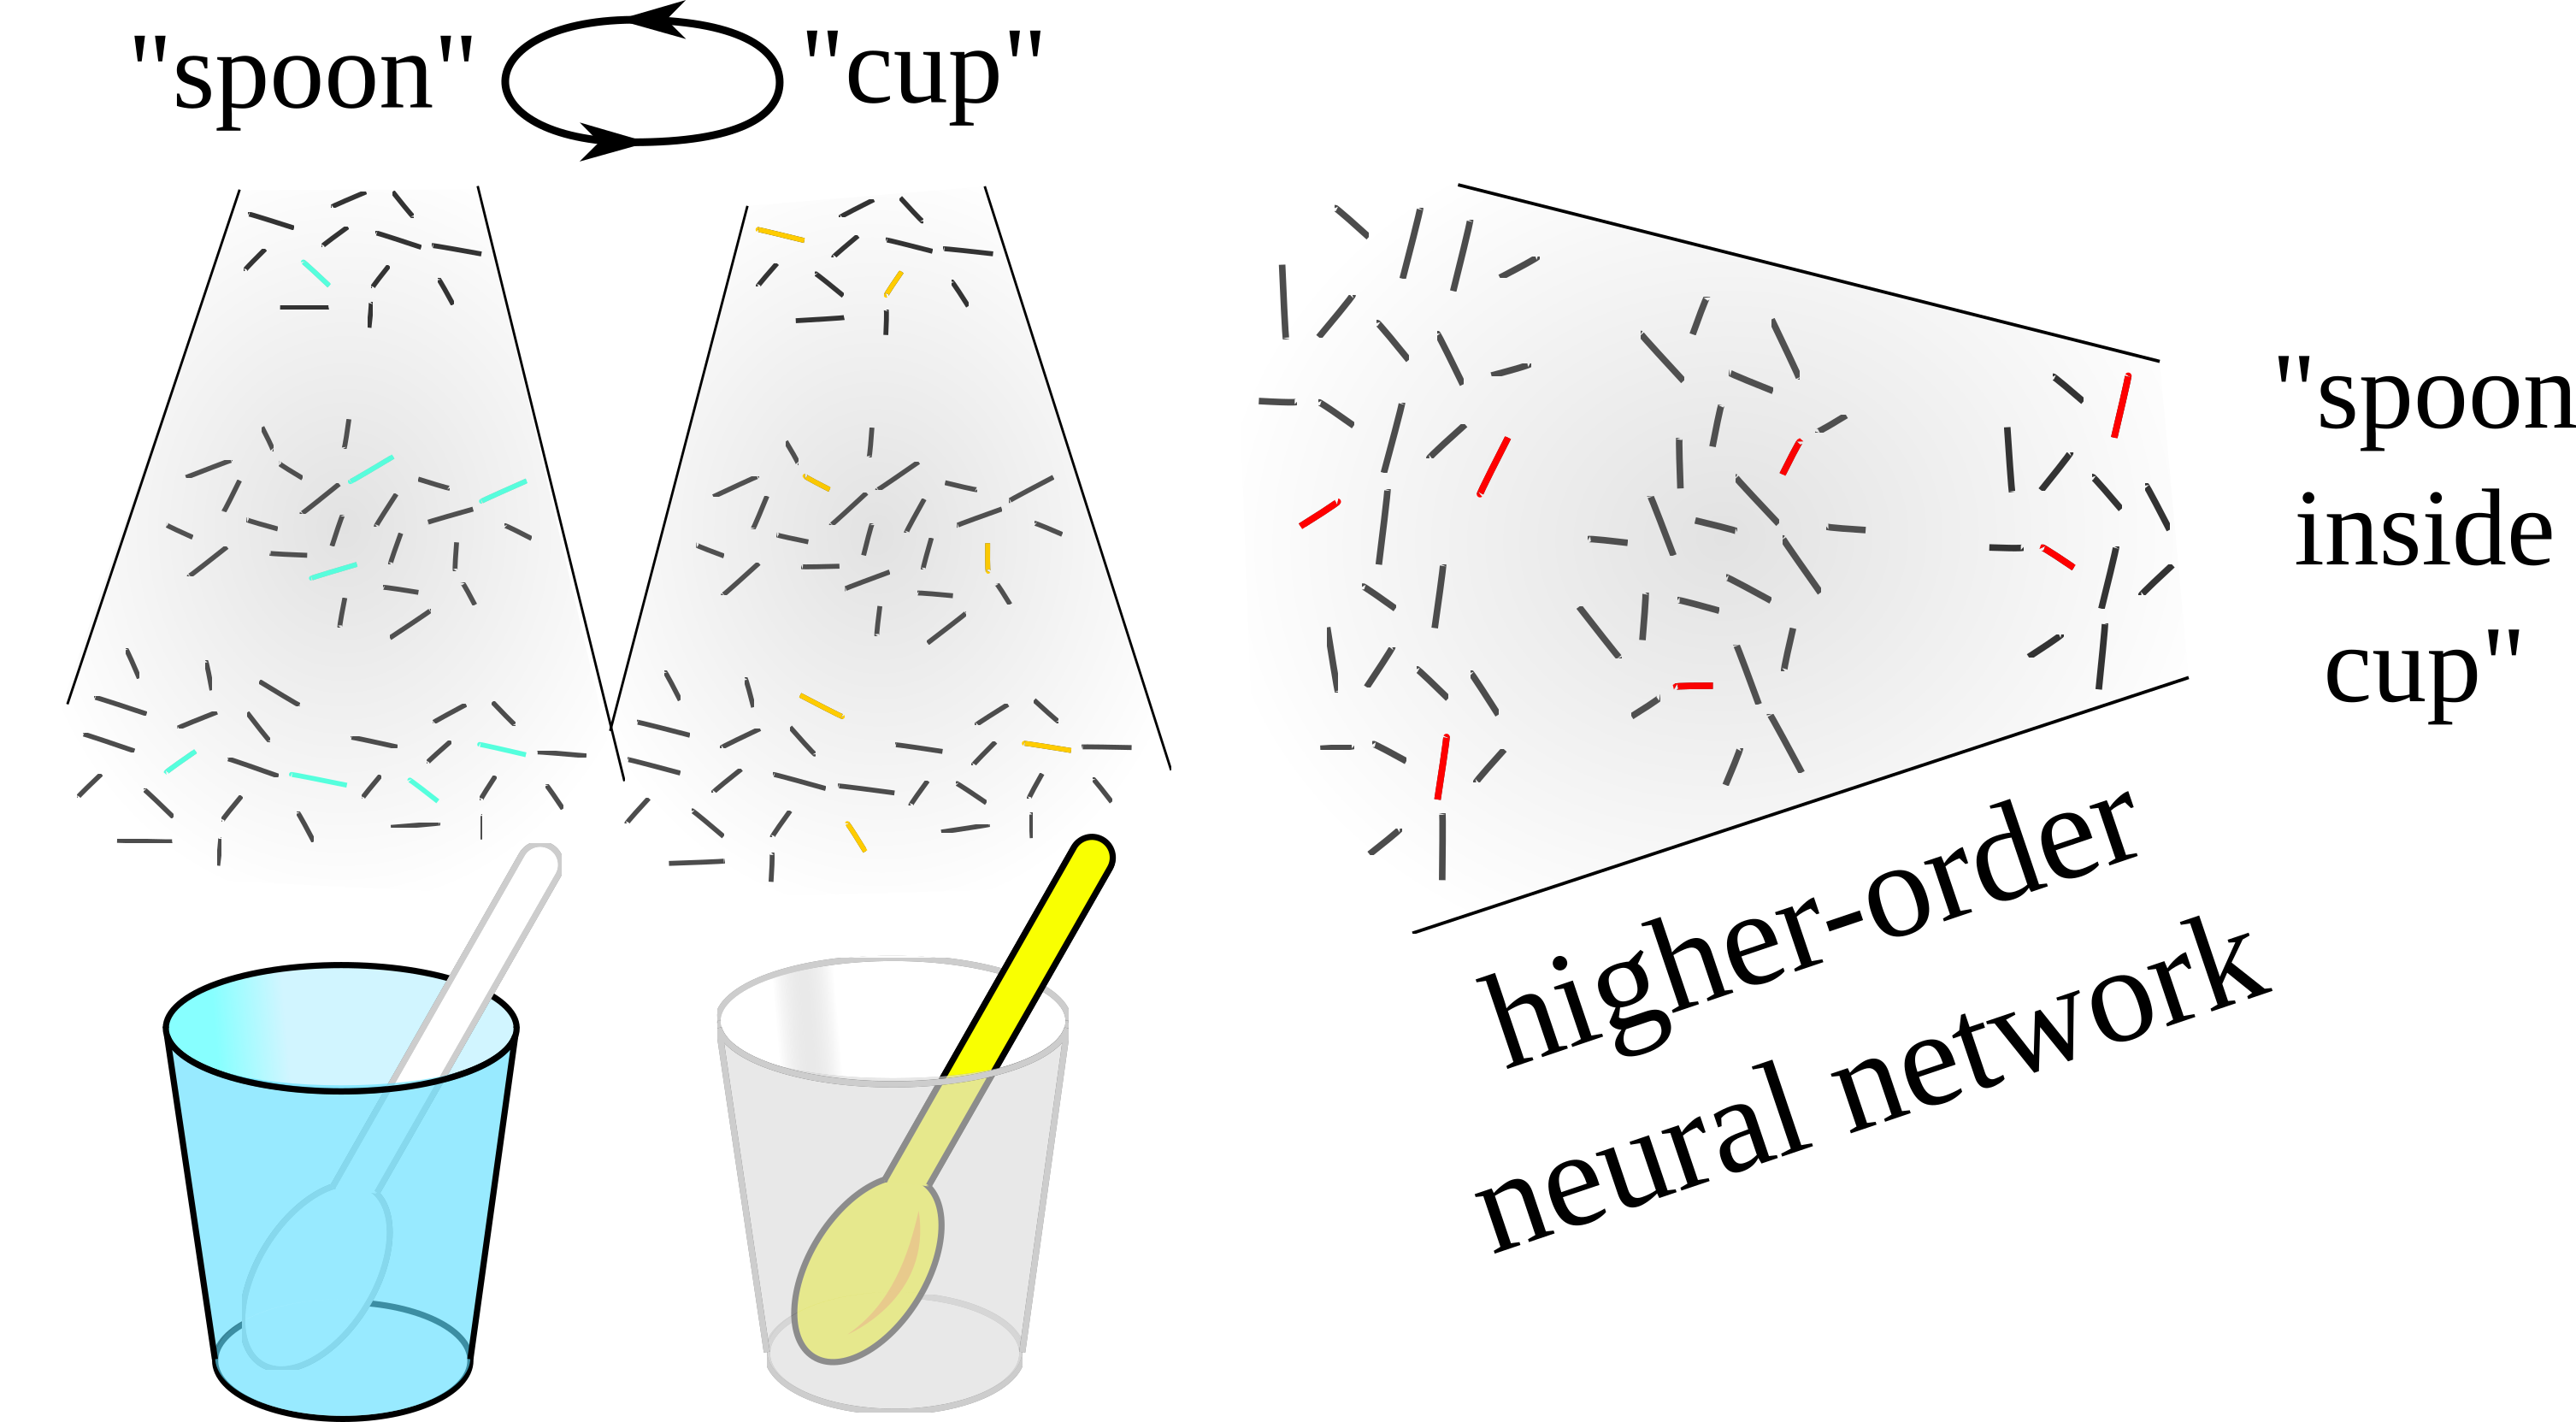
\includegraphics[scale=0.5]{higher-order-NN.png}}}
	\end{equation}
	
	\item 这似乎是一个 $\mbox{特征空间} \times \mbox{时间}$ 的映射 $f: X \times T \rightarrow Y$
	
	\item {\color{red}关於这部分其实我仍未肯定,或许有其他方法}
\end{itemize}
\end{frame}

\begin{comment}
\begin{frame}
\frametitle{神经 $\leftrightarrow$ 逻辑 correspondence}
\begin{itemize}
	\item 我们的目标是了解 神经表示 和 逻辑表示 之间的关系,这关系或许可以用范畴论描述?
	
	\item 定义 复杂情境 (complex scenario) 是 感知材料 (sensory data) 的一个片段,如:
	\begin{equation}
		\vcenter{\hbox{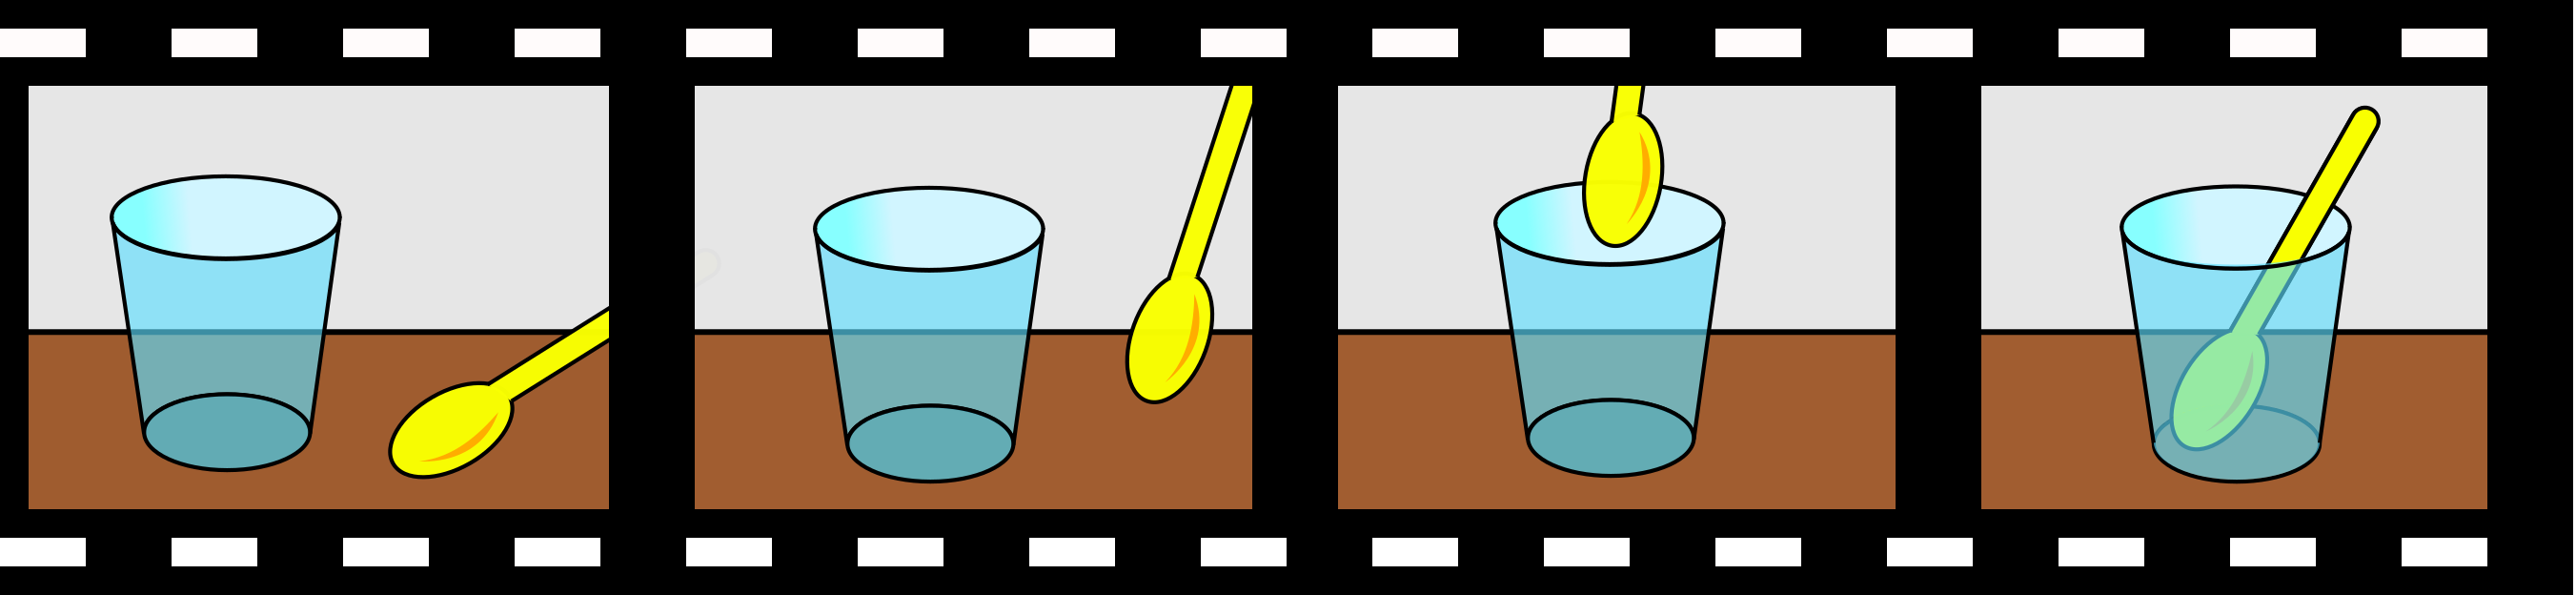
\includegraphics[scale=0.5]{sensory-movie.png}}}
	\end{equation}
	又或者一个故事,例如「John 爱 Mary 但 Mary 不爱他」
	
	\item 一个复杂情境 可以用若干个 特征簇 描述
	
	\item Equivalently, 复杂情境 可以用 \emp{逻辑} 表示,就是一大堆 逻辑命题 的 conjunction,这些命题 钜细无遗 地描述该情境
\end{itemize}
\end{frame}
\end{comment}

\begin{frame} %[allowframebreaks] this option seems to cause error!!
\frametitle{References}
\cc{多谢收看}{Thanks for watching} \smiley \\
\nocite{Goldblatt1984}
\nocite{MacLane1992}
\nocite{Streicher2006}
\nocite{Awodey2006}
\nocite{Jacobs1999}
\nocite{Abramsky2011}
\nocite{Caramello2018}
\nocite{Lawvere1997}
\nocite{Lawvere2003}
\nocite{Rodin2014}
\nocite{Vickers1989}
\nocite{Pitts1991}
\nocite{Sorensen2006}
% \nocite{Hindley1997}

\printbibliography
\end{frame}

\end{document} 